\documentclass[11pt]{scrartcl}

% packages

% \usepackage{blindtext}

\usepackage[utf8]{inputenc}
\usepackage[T1]{fontenc}
\usepackage[english]{babel}

\usepackage[top=30mm, bottom=30mm, left=20mm, right=20mm]{geometry}
\usepackage{fancyhdr}
\usepackage{setspace}
\usepackage{parskip}

\usepackage{graphicx}
\usepackage[section]{placeins}
\usepackage[table, dvipsnames]{xcolor}
\usepackage{pdfpages}

\usepackage{hyperref}
\usepackage[labelfont=bf]{caption}

\usepackage[round]{natbib}

\usepackage{listings}
\usepackage{minted}
\usepackage{algorithmicx}
\usepackage[noend]{algpseudocode}
\usepackage{algorithm}

\usepackage{tabularx}
\usepackage{multirow}
\usepackage{multicol}
\usepackage{caption}
\usepackage{subcaption}
\usepackage{adjustbox}

\usepackage{amsmath, amssymb}

%%%%%%%%%%%%%%%%%%%%%% preamble %%%%%%%%%%%%%%%%%%%%%%

\renewcommand*{\sectionmark}[1]{ \markright{\thesection\ ##1} }
% \renewcommand*{\chaptermark}[1]{ \markboth{\chaptername\ \thechapter: ##1}{} }
\fancyhead[LE,RO]{\thepage}
\fancyhead[LO,RE]{}
\fancyfoot{}
\pagestyle{fancy}

\definecolor{myblue}{RGB}{46, 59, 160}

\graphicspath{{pics/}}

\hypersetup{
	pdfstartpage=7,
    pdfstartview = FitB,
	pdfpagelayout=SinglePage,
	pdftitle={Project Report},
	pdfsubject={Statistical Learning Theory},
	pdfauthor={Maurice Wenig},
	pdfcreator={Maurice Wenig},
	pdfproducer={Maurice Wenig},
	pdfkeywords={meta, information, pdf, hyperref, latex},
	colorlinks=true,
	linkcolor=myblue,
	citecolor=myblue
}

\bibliographystyle{unsrtnat}

\newcommand*\justify{%
  \hyphenchar\font=`\-% allowing hyphenation
}

\definecolor{line_number_colour}{rgb}{0.5,0.5,0.5}
\renewcommand\theFancyVerbLine{\color{line_number_colour}\tiny\arabic{FancyVerbLine}}
\setminted[C]{
	% linenos, 
	breaklines,
	fontsize=\footnotesize
}

\hyphenpenalty=5000
\tolerance=5000

% TODO: remove for digital version
% \selectcolormodel{gray}

%----- new commands
\newcommand{\Romannumeral}[1]{\MakeUppercase{\romannumeral #1}}
\newcommand{\set}[1]{\{#1\}}
\newcommand{\abs}[1]{\left\vert #1 \right\vert}
\newcommand{\norm}[1]{\left\| #1 \right\|}
\newcommand{\skal}[2]{\left\langle #1 | #2 \right\rangle}
\newcommand{\script}[1]{
    skripte/aufgabe#1.py
    \lstinputlisting{skripte/aufgabe#1.py}
}
%----- defs
\def\notiff{\mathrel{{\ooalign{\hidewidth$\not\phantom{"}$\hidewidth\cr$\iff$}}}}
\def\R{\mathbb{R}}
\def\bbone{\text{\usefont{U}{bbold}{m}{n}1}}
\def\1{\mathbb{1}}
\def\T{\top}
\def\ndy{
    \textcolor{red} {\hfill not done yet!}
    \reversemarginpar
    \marginpar{\raggedleft\textcolor{red}{\rule{2mm}{2mm}}}
}
\def\ghostline{\hfill\vspace*{-5mm}}

%%%%%%%%%%%%%%%%%%%%%% main %%%%%%%%%%%%%%%%%%%%%%

\begin{document}

\thispagestyle{empty}
\begin{center}
	\begin{LARGE}
		\textbf{Statistical Learning Theory LAB}
	\end{LARGE}\vspace{3mm}\\
	\begin{Large}
		\textbf{Project Report}
	\end{Large}\vspace{5mm}\\
	\begin{large}
		Maurice Wenig
	\end{large}
\end{center}
% \setcounter{tocdepth}{1}
\tableofcontents
\clearpage

% algorithm, its performance, technical details, your score
% In the report focus on the key features of your system.
% Especially if you do not implement the used algorithms yourself make sure to cover them in the report so its clear you could have implemented them yourself
% (i.e. someone could implement the algorithm only reading your report).
% If you combine several predictors, you should describe at least two of them in detail, for the others the basics should be enough.

\fancyhead[LO,RE]{\itshape\nouppercase\leftmark}
\section{Algorithms}
\subsection[Neighbourhood]{Neighbourhood-Based Recommenders}
\subsubsection[User-Based]{User-Based Recommender}
% include long tail plot
The user-based recommender compares users based on their rated items. An item rating from a user is then predicted based on ratings of that item from similar users.
The similarity measure used to compare users is Pearson:
$$\text{Sim}(u, v) = \frac{\sum\limits_{i\in I_{uv}} w_i \cdot s_{ui} s_{vi}}{\sqrt{\sum\limits_{i\in I_{uv}} w_i \cdot  s_{ui}} \cdot \sqrt{\sum\limits_{i\in I_{uv}} w_i \cdot  z_{vi}}}$$
where $I_{uv}$ are the items that both users $u$ and $v$ have rated, $s_{ui} = r_{ui} - \mu_u$ is the centered rating from user $u$.
The mean rating $\mu_u$ can be calculated individually for every comparison, based on only the common items, or it can be calculated once for every user, based on all their rated items.
$w_i = \log\frac{\text{\# users}}{\text{\# users who rated } i}$ are item weights to combat the impact of the long tail in the number of item ratings.

To prefer users with more common items, the similarites of users with less than $\beta$ common items are made smaller.
$$\text{Sim}(u, v) \gets \text{Sim}(u, v) \cdot \frac{\min\set{\abs{I_{uv}}, \beta}}{\beta}$$

The hyper parameter $\alpha$ can be used to amplify the importance of similarity.
$$\text{Sim}(u, v) \gets \text{Sim}(u, v)^\alpha$$

Based on these similarities, a peer group $P_u(i)$ of users is determined. For this, the users are sorted by similarity.
To improve efficiency in the online phase, the sorting is done in the offline phase.
For this, the similarities between every user $u, v$ are saved in the similarity matrix.
The order of peers for a specific user is then determined by sorting the respective row vector.

In the online phase, this order is simply applied. Users are then removed, if they have not rated them item $i$, or their similarity to user $u$ is below a certain threshold $S_{min}$.
The top $k$ remaining users are then the peer group $P_u(i)$.

The predicted item rating from a user is then calculated as a sum of ratings from similar users, weighted with their relative similarity.
The means and variances of the user ratings are normalized to not influence the prediction.
$$\hat{r}_{ui} = \mu_u + \sigma_u \cdot \frac{\sum\limits_{v \in P_u(i)} \text{Sim}(u, v) \cdot z_{vi}}{\sum\limits_{v \in P_u(i)} \abs{\text{Sim}(u, v)}}$$
where $z_{ui} = s_{ui} / \sigma_u$ is the normalized rating, $\sigma_u$ the variance of the ratings of user $u$.
If the user has only ever given one distinct rating, the variance is set to an arbitrary value of 1.

\hypertarget{special_cases}{}
In special cases where the user or the item has never been seen before, similarities can not be calculated. In those special cases, the ratings were predicted in a different way:
\begin{itemize}
	\item user and item unknown: predict average between minimum and maximum possible rating
	\item user unknown, item known: predict average rating of that item
	\item user known, item unknown: predict average rating of that user
\end{itemize}
Also, if the original item rating of the user is known, this original rating can be predicted.

\subsubsection[Item-Based]{Item-Based Recommender}
The item-based recommender compares items based on their user ratings. An item rating from a user is then predicted based on ratings of similar items from that user.
It functions very similar to the user-based recommender. The similarity function is adapted to still use user means $\mu_u$ instead of item means $\mu_i$ to normalize user preferences.
The predicted rating is then a weighted sum of similar items, the user has rated.

$$\hat{r}_{ui} = \frac{\sum\limits_{j \in P_i(u)} \text{Sim}(i, j) \cdot r_{uj}}{\sum\limits_{j \in P_i(u)} \abs{\text{Sim}(i, j)}}$$

\subsubsection{Clustering}
To increase efficiency, the users/items can be clustered before the creation of the similarity matrix. This way, only users/items that are in the same cluster have to be compared.

This is done using an adapted version of K-means.
To account for the sparsity of the rankings matrix, the entries of the mean of a cluster are calculated using only vectors, where the entries are not missing in the respective dimensions.
The distance measure is also adapted. The distance between two vectors is calculated only with the common dimensions, where ratings are not missing.
The result is then divided by the number of common dimensions to get a distance measure that is independent of the number of common dimensions.


\subsection[Factorization]{Factorization-Based Recommender}
In the factorization-based recommender, the users and items are assumed to be in a common latent factor space $R^f$ of user preferences $q_i$ and item characteristics $p_u$.
The rating $r_{ui}$ is then modelled as the user's interest in the item's characteristics. User and item biases are also taken into account.
$$\hat{r}_{ui} = q_i^\T p_u + \mu + b_i + b'_u$$

The goal is then to learn the factors $q_i, p_u$, such that the squared error function on the ratings of the training set is minimal.
$$\min\limits_{p, q, b} \sum\limits_{(u, i) \in \kappa} (r_{ui} - \hat{r}_{ui})^2 + \lambda \left(\norm{q_i}^2 + \norm{p_u}^2 + b_i^2 + {b'_u}^2\right)$$
with $\kappa$ as the set of $(u, i)$ pairs in the training set, $\lambda$ as the regularization parameter.

To achieve this minimzation, alternating least squares is used.
$q, p$ are initiated randomly.
Then, in each step, one of them is fixed and the other one is solved optimally.
This is done until the change of the vectors in $q, p$ is below a threshold $\epsilon$ or a maximum number of iterations is reached.

To optimally solve the minimization at each step, ridge regression is used.
Because they are independent, each of the summands are optimized individually.
\begin{gather*}
	\min\limits_{p_u, b'_u} \sum\limits_{i \in \kappa_u} \left((r_{ui} - b_i - \mu) - (q_i^\T p_u + b'_u)\right)^2 + \lambda \left(\norm{p_u}^2 + {b'_u}^2\right)\\
	\min\limits_{q_i, b_i} \sum\limits_{u \in \kappa_i} \left((r_{ui} - b'_u - \mu) - (q_i^\T p_u + b_i)\right)^2 + \lambda \left(\norm{q_i}^2 + b_i^2\right)
\end{gather*}
with $\kappa_u$ as the set of items that have been rated by $u$, $\kappa_i$ as the set of user that have rated $i$.

The ridge regression the boils down to solving the regularized normal equations:
\begin{gather*}
	\left(Q_{\kappa_u} {Q_{\kappa_u}}^\T + \lambda\bbone\right) p_u = Q_{\kappa_u} y_{\kappa_u}\\
	\left(P_{\kappa_i} {P_{\kappa_i}}^\T + \lambda\bbone\right) q_i = P_{\kappa_i} y_{\kappa_i}
\end{gather*}
with
\begin{align*}
	Q_{\kappa_u}  & = (q_{i_1}, \dots, q_{i_n})                                  \\
	y_{\kappa_u}  & = \vec{r}_{\kappa_u} - \vec{b}                               \\
	              & = (r_{ui_1}, \dots, r_{ui_n})^\T - (b_{i_1}, \dots, b_{i_n}) \\
	i, \dots, i_n & \in \kappa_u
\end{align*}
for determining $p_u$ and
\begin{align*}
	P_{\kappa_i}    & = (p_{u_1}, \dots, p_{u_n})                                      \\
	y_{\kappa_i}    & = \vec{r}_{\kappa_i} - \vec{b'}                                  \\
	                & = (r_{u_1 i}, \dots, r_{u_n i})^\T - (b'_{u_1}, \dots, b'_{u_n}) \\
	u_1, \dots, u_n & \in \kappa_i
\end{align*}
for determining $q_i$.


The biases can either be fixed or part of the optimization.
If the biases are fixed, $\mu$ is the overall mean rating in the training set, $b'_u = \mu_u - \mu$ is the mean user rating centered around the overall mean rating, $b_i = \mu_i - \mu$ is the mean item rating centered around the overall mean rating.
If the biases are part of the optimization, they are the affine part of the ridge regression at each step.
This affine part can be obtained by appending a constant 1 to the training vectors and reading its respective coefficient.

The special cases are handled in the same way as they are in the \hyperlink{special_cases}{User Based Recommender}.

\subsection[Hybrid]{Hybrid Recommender}
The hybrid combines an array of $K$ recommenders. The predictions are a linear combination of the predictions of those recommenders.
$$\hat{r}_{ui} = \sum\limits_{k = 1}^{K} \alpha_k \hat{r}^{(k)}_{ui} = \vec{\alpha}^\T \vec{r}_{ui}$$

To learn $\vec{\alpha}$, the training set is separated into two parts: a fitting set, and a held out set.
The recommenders are then trained on the fitting set.
Then, the recommenders predict the labels of the held out set.
The optimal alpha can either minimize the mean absolute error
$$\mathcal{E}_1 = \frac{1}{m}\norm{R - \vec{R} \vec{\alpha}}_1$$
or the (half) mean squared error
$$\mathcal{E}_2 = \frac{1}{2m}\norm{R - \vec{R} \vec{\alpha}}^2_2$$
$m$ as the number of samples in the held out set,
$R = (r_1, \dots, r_m)^\T$ as the vector of true ratings of the held out samples,
$\vec{R} = (\vec{r}_1, \dots, \vec{r}_m)^\T$ as the matrix of predictions on the held out samples.

$\vec{\alpha}$ is then optimized with gradient descent. Every entry is intialized with $\frac{1}{K}$.
At each step, $\vec{\alpha} \gets \vec{\alpha} - \gamma \nabla\mathcal{E}(\vec{\alpha})$ is pushed into the direction of the negative gradient of the error, scaled with a learning rate $\gamma$.
This is done until the error changes less than a threshold $\epsilon$, or the maxmimum amount of iterations is reached.
\begin{align*}
	\nabla\mathcal{E}_1(\vec{\alpha}) & = \frac{1}{m} \text{sign}\left(R - \vec{R} \vec{\alpha}\right)^\T \vec{R} \\
	\nabla\mathcal{E}_2(\vec{\alpha}) & = \frac{1}{m} \left(R - \vec{R} \vec{\alpha}\right)^\T \vec{R}
\end{align*}

After $\vec{\alpha}$ has been determined, the predictors are trained on the whole training set to not miss out on information.
Special cases do not need to be handled, as they are handled in the individual recommenders.

\clearpage
\section{Results}
% include plot: didn't improve much from equally distributed weights
% also talk about hyper parameters
The hyper parameters were tuned based on the root mean squared error and the mean absolute error from cross validation.
Those were the best performing ones:
\begin{itemize}
	\item user based: \begin{itemize}
		      \item $k = 50$ neighbours in peer group
		      \item $\alpha = 1$, not amplifying importance of similarity
		      \item $S_{min} = 0.4$ minimum similarity
		      \item $\beta = 4$ common dimensions before similarity reduction
		      \item 8 clusters
	      \end{itemize}
	\item item based: \begin{itemize}
		      \item $k = 50$ neighbours in peer group
		      \item $\alpha = 1$, not amplifying importance of similarity
		      \item $S_{min} = 0.6$ minimum similarity
		      \item $\beta = 6$ common dimensions before similarity reduction
	      \end{itemize}
	\item factorization based: \begin{itemize}
		      \item $\lambda = 5$ regularization parameter
		      \item $f = 20$ latent dimensions
		      \item biases not fixed
		      \item $\epsilon = 10^{-2}$, max 20 iterations
	      \end{itemize}
	\item hybrid of user based, item based, factorization based: \begin{itemize}
		      \item $\gamma = 1$ learning rate
		      \item $\epsilon = 10^{-4}$, max 100 iterations
	      \end{itemize}
\end{itemize}
\begin{figure}[!htb]
	\centering
	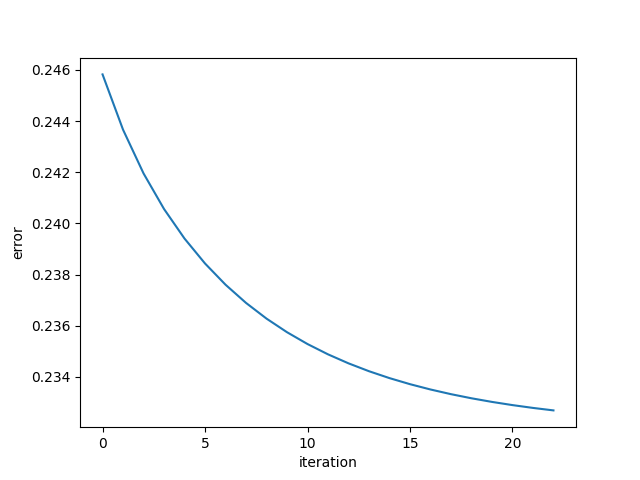
\includegraphics[scale=0.4]{../plots/descent.png}
	\caption{Hybrid error during gradient descent}\label{fig:hybrid_descent}
\end{figure}
It is worthy to note that the hybrid didn't improve much compared to the initial equal weights.
In \autoref{fig:hybrid_descent} you can see mean absolute error of the hybrid recommender during the gradient descent of $\vec{\alpha}$.

\subsection{Performance}
For time measurement, the recommenders were trained on \href{run:../input/train.csv}{\texttt{train.csv}} (435K samples) and evaluated on \href{run:../input/qualifying_blanc.csv}{\texttt{qualifying\_blanc.csv}} (109K samples).
\begin{table}[!htb]
	\centering
	\rowcolors{2}{gray!25}{white}
	\begin{tabular}{|l|c|c|}
		\hline
		Recommender   & offline phase & online phase \\\hline\hline
		user based    & 15.97s        & 6.84s        \\\hline
		item based    & 44.3s         & 4.79s        \\\hline
		factorization & 85.65s        & 0.53s        \\\hline
		hybrid        & 304.1s        & 26.79s       \\\hline
	\end{tabular}
	\caption{Runtime in offline and online phase}\label{tab:performance}
\end{table}

\subsection{Error Scores}
The error scores were measured with cross validation on the training set, with $R = 8$ rotations.
Root mean squared error (rmse) and mean absolute error (mae) were calculated.
\begin{table}[!htb]
	\centering
	\rowcolors{2}{gray!25}{white}
	\begin{tabular}{|l|c|c|}
		\hline
		Recommender   & rmse  & mae   \\\hline\hline
		user based    & 0.670 & 0.301 \\\hline
		item based    & 0.569 & 0.222 \\\hline
		factorization & 0.559 & 0.233 \\\hline
		hybrid        & 0.513 & 0.202 \\\hline
	\end{tabular}
	\caption{Error scores}\label{tab:errors}
\end{table}
\subsection{Final Score}
My final score on the \href{http://csujena.pythonanywhere.com/}{validation set} is 0.530.
It was achieved with the hybrid recommender.


% \typeout{}
% \clearpage
% \pagestyle{empty}
% \bibliography{literatur}
% \listoffigures
% \listoftables
% \appendix
% \input{chapters/Anhang}

\end{document}